\documentclass[]{report}
\usepackage{lmodern}
\usepackage{amssymb,amsmath}
\usepackage{ifxetex,ifluatex}
\usepackage{fixltx2e} % provides \textsubscript
\ifnum 0\ifxetex 1\fi\ifluatex 1\fi=0 % if pdftex
  \usepackage[T1]{fontenc}
  \usepackage[utf8]{inputenc}
\else % if luatex or xelatex
  \ifxetex
    \usepackage{mathspec}
  \else
    \usepackage{fontspec}
  \fi
  \defaultfontfeatures{Ligatures=TeX,Scale=MatchLowercase}
\fi
% use upquote if available, for straight quotes in verbatim environments
\IfFileExists{upquote.sty}{\usepackage{upquote}}{}
% use microtype if available
\IfFileExists{microtype.sty}{%
\usepackage{microtype}
\UseMicrotypeSet[protrusion]{basicmath} % disable protrusion for tt fonts
}{}
\usepackage{hyperref}
\hypersetup{unicode=true,
            pdftitle={PROJECT 2: PREDICTING PH},
            pdfauthor={Juliann McEachern},
            pdfborder={0 0 0},
            breaklinks=true}
\urlstyle{same}  % don't use monospace font for urls
\usepackage{graphicx,grffile}
\makeatletter
\def\maxwidth{\ifdim\Gin@nat@width>\linewidth\linewidth\else\Gin@nat@width\fi}
\def\maxheight{\ifdim\Gin@nat@height>\textheight\textheight\else\Gin@nat@height\fi}
\makeatother
% Scale images if necessary, so that they will not overflow the page
% margins by default, and it is still possible to overwrite the defaults
% using explicit options in \includegraphics[width, height, ...]{}
\setkeys{Gin}{width=\maxwidth,height=\maxheight,keepaspectratio}
\IfFileExists{parskip.sty}{%
\usepackage{parskip}
}{% else
\setlength{\parindent}{0pt}
\setlength{\parskip}{6pt plus 2pt minus 1pt}
}
\setlength{\emergencystretch}{3em}  % prevent overfull lines
\providecommand{\tightlist}{%
  \setlength{\itemsep}{0pt}\setlength{\parskip}{0pt}}
\setcounter{secnumdepth}{0}

%%% Use protect on footnotes to avoid problems with footnotes in titles
\let\rmarkdownfootnote\footnote%
\def\footnote{\protect\rmarkdownfootnote}

%%% Change title format to be more compact
\usepackage{titling}

% Create subtitle command for use in maketitle
\providecommand{\subtitle}[1]{
  \posttitle{
    \begin{center}\large#1\end{center}
    }
}

\setlength{\droptitle}{-2em}

  \title{PROJECT 2: PREDICTING PH}
    \pretitle{\vspace{\droptitle}\centering\huge}
  \posttitle{\par}
    \author{Juliann McEachern}
    \preauthor{\centering\large\emph}
  \postauthor{\par}
      \predate{\centering\large\emph}
  \postdate{\par}
    \date{10 December 2019}

% set plain style for page numbers
\usepackage[margin=1in]{geometry}
\usepackage{fancyhdr}
\pagestyle{fancy}
\fancyhead[LE,RO]{\textbf{Group 2}}
\fancyhead[RE,LO]{\textbf{Project 2: Predicting PH}}
\raggedbottom
\setlength{\parskip}{1em}

% change font
\usepackage{fontspec}
\setmainfont{Arial}

% format titles 
\usepackage{xcolor}
\usepackage{sectsty}
\usepackage{etoolbox}
\usepackage{titling}
\definecolor{prettyblue}{RGB}{84, 144, 240}
\definecolor{bluegray}{RGB}{98, 107, 115}
\pretitle{\begin{center}\Huge\color{prettyblue}\textbf}
\posttitle{\par\LARGE\color{gray}DATA 624 - Predictive Analytics\linebreak Group 2\end{center}}
\preauthor{\begin{center}\large\textbf{Group Members:}\linebreak\textit}
\postauthor{\end{center}}

% Format chapter output
\usepackage{titlesec}
\titleclass{\part}{top}
\titleclass{\chapter}{straight}
\titleformat{\chapter}
  {\normalfont\color{prettyblue}\LARGE\bfseries}{\thechapter}{1em}{}
\titlespacing*{\chapter}{0pt}{3.5ex plus 1ex minus .2ex}{2.3ex plus .2ex}


% create color block quotes
\usepackage{tcolorbox}
\newtcolorbox{myquote}{colback=purple!05!white, colframe=purple!75!black}
\renewenvironment{quote}{\begin{myquote}}{\end{myquote}}

% kable 
\usepackage{tabu}
\usepackage{float} 

% multicolumn
\usepackage{multicol}

% bullets
\newenvironment{tight_enumerate}{
\begin{enumerate}
  \setlength{\itemsep}{0pt}
  \setlength{\parskip}{0pt}
  }{\end{enumerate}}
  
\newenvironment{tight_itemize}{
\begin{itemize}
  \setlength{\topsep}{0pt}
  \setlength{\itemsep}{0pt}
  \setlength{\parskip}{0pt}
  \setlength{\parsep}{0pt}
  }{\end{itemize}}

\usepackage{paralist}

%hyperlink
\usepackage{hyperref}
\hypersetup{
    colorlinks=true,
    linkcolor=bluegray,
    filecolor=magenta,      
    urlcolor=cyan}
\usepackage{booktabs}
\usepackage{longtable}
\usepackage{array}
\usepackage{multirow}
\usepackage{wrapfig}
\usepackage{float}
\usepackage{colortbl}
\usepackage{pdflscape}
\usepackage{tabu}
\usepackage{threeparttable}
\usepackage{threeparttablex}
\usepackage[normalem]{ulem}
\usepackage{makecell}
\usepackage{xcolor}

\begin{document}
\maketitle

{
\setcounter{tocdepth}{1}
\tableofcontents
}
\thispagestyle{empty}
\newpage
\clearpage
\pagenumbering{arabic}

\hypertarget{intro}{%
\chapter*{Introduction}\label{intro}}
\addcontentsline{toc}{chapter}{Introduction}

This project is designed to evaluate production data from a beverage
manufacturing company. Our assignment is to predict \texttt{PH}, a Key
Performance Indicator (KPI), with a high degree of accuracy through
predictive modeling. After thorough examination, we approached this task
by splitting the provided data into training and test sets. We evaluated
several models on this split and found that
\textbf{what-ever-worked-best} method yielded the best results.

Each group member worked individually to create their own solution. We
built our final submission by collaboratively evaluating and combining
each others' approaches. Our introduction should further outline
individual responsibilities. For example, \textbf{so-and-so} was
responsible for \textbf{xyz task}.

For replication and grading purposes, we made our code avaliable in the
appendix section. This code, along with the provided data, score-set
results, and individual contributions, can also be accessed through our
group github repository:

\begin{compactitem}
  \item \href{https://github.com/JeremyOBrien16/CUNY_DATA_624/tree/master/Project_Two}{Pretend I'm a working link to R Source Code}
  \item \href{https://github.com/JeremyOBrien16/CUNY_DATA_624/tree/master/Project_Two}{Pretend I'm a working link to Provided Data}
  \item \href{https://github.com/JeremyOBrien16/CUNY_DATA_624/tree/master/Project_Two}{Pretend I'm a working link to Excel Results}
  \item \href{https://github.com/JeremyOBrien16/CUNY_DATA_624/tree/master/Project_Two}{Pretend I'm a working link to Individual Work}
\end{compactitem}

\hypertarget{data-exploration}{%
\chapter{Data Exploration}\label{data-exploration}}

The beverage manufacturing production dataset contained 33
columns/variables and 2,571 rows/cases. In our initial review, we found
that the response variable, \texttt{PH}, had four missing observations.
We choose to drop the complete cases of the observations with null data
in the target as they accounted for such a small proportion (\textless{}
0.002\%) of the observations.

We also identified that 94\% of the predictor variables had missing data
points. Despite this high occurance, the NA values in the majority of
these predictors accounted for less than 1\% of the total observations.
Only eleven variables, highlighted in the plot below, were missing more
than 1\% of data:

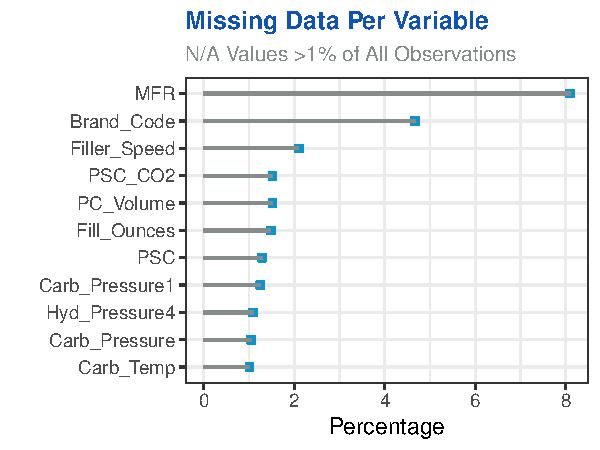
\includegraphics{Proj2-JM_files/figure-latex/unnamed-chunk-1-1.pdf}

Without additional data regarding production, we assume that the
\texttt{NA} values are missing at random. We applied a Multiple
Imputation by Chained Equations (MICE) algorthim, which uses sequential
regression to create multiple imputations across all the incomplete
cases (including categorical data).

\hypertarget{predictor-variables}{%
\section{Predictor Variables}\label{predictor-variables}}

\hypertarget{response-variable}{%
\section{Response Variable}\label{response-variable}}

Understanding the influence PH has on our predictors is key to building
an accurate predictive model. PH is a measure of acidity/alkalinity that
must conform in a critical range.

\hypertarget{data-transformations}{%
\section{Data Transformations}\label{data-transformations}}

Text text text.

\hypertarget{predictive-modeling}{%
\chapter{Predictive Modeling}\label{predictive-modeling}}

Text text.

\hypertarget{train}{%
\section{Train}\label{train}}

Train text.

\hypertarget{test}{%
\section{Test}\label{test}}

Test text.

\hypertarget{discussion}{%
\chapter{Discussion}\label{discussion}}

Eval text. The end.

\hypertarget{conclusion}{%
\chapter{Conclusion}\label{conclusion}}

sfasdfs

\hypertarget{Appendix}{%
\chapter*{Appendix}\label{Appendix}}
\addcontentsline{toc}{chapter}{Appendix}

Code \& stuff here.


\end{document}
